\documentclass[a4paper,11pt]{article}
\pdfoutput=1 % if your are submitting a pdflatex (i.e. if you have
             % images in pdf, png or jpg format)

\usepackage{jheppub} % for details on the use of the package, please
                     % see the JHEP-author-manual

\usepackage[T1]{fontenc} % if needed



\title{\boldmath Notes on Pairs Trading}


%% %simple case: 2 authors, same institution
%% \author{A. Uthor}
%% \author{and A. Nother Author}
%% \affiliation{Institution,\\Address, Country}

% more complex case: 4 authors, 3 institutions, 2 footnotes
\author{Elliot Golias,\note{Corresponding author.}}
%\author[c]{S. Econd,}
%\author[a,2]{T. Hird\note{Also at Some University.}}
%\author[a,2]{and Fourth}

% The "\note" macro will give a warning: "Ignoring empty anchor..."
% you can safely ignore it.

\affiliation[a]{Case Western Reserve University,\\some-street, Country}
%\affiliation[b]{Another University,\\different-address, Country}
%\affiliation[c]{A School for Advanced Studies,\\some-location, Country}

% e-mail addresses: one for each author, in the same order as the authors
\emailAdd{elliotgolias@case.edu}
%\emailAdd{second@asas.edu}
%\emailAdd{third@one.univ}
%\emailAdd{fourth@one.univ}




%\abstract{Abstract...}



\begin{document} 
\maketitle
\flushbottom

\section{Introduction}
\label{sec:intro}

A basic pairs trading strategy consists of exploiting an out-of-equilibrium market; if two assets typically trade at some spread, then the narrowing/widening of the spread between the assets may be exploited for profit
For example, if the spread widens, then one should buy the low asset and short the high asset. On the other hand, if the spread narrows, than one should short the higher asset and buy the lower asset. 

Consider a state process $\{x_k\}$, where $x_k$ denotes the value of a real variable at the time $t_k = k \tau$, where $\tau$ is the separation between times and $k=0, 1, 2, \dots$. We assume that $\{ x_k \}$ is mean-reverting, meaning we have the following relation between the spread of susequent pairs of $x_k$:
%
\begin{align}
	x_{k+1} - x_k = (a-b x_k) \tau + \sigma \sqrt{\tau} \varepsilon_{k+1},
\end{align}
%
where $\sigma \geq 0, b > 0, a \in \mathbf{R}$, and $\{ \varepsilon_k \}$ is iid Gaussian $\mathcal{N}(0, 1)$ and independent of ${x_k}$. With this definition, the process reverts to $\mu = a/b$ with \textit{strength} $b$. This implies that
%
\begin{align}
	x_k \sim \mathcal{N}(\mu_k, \sigma_k^2),
\end{align}
%
where
%
\begin{align}
	\mu_k = \frac{a}{b} +\left[\mu_0 - \frac{a}{b} \right](1 - b \tau)^k,
\end{align}
%
and
%
\begin{align}
	\sigma_k^2 = \frac{\sigma^2 \tau}{1-(1-b \tau)^2} \left [ 1-(1-b\tau)^{2k} \right] + \sigma_0^2 (1-b \tau)^{2k}
\end{align}
%
We can also express the mean reversion condition in the form
%
\begin{align}
	x_{k+1} = A + B x_k + C \varepsilon_{k+1},
\end{align}
%
where $A = a \tau \geq 0, 0 < B = 1- b \tau$ and $C = \sigma \sqrt{\tau}$.
\begin{figure}[tbp]
\centering % \begin{center}/\end{center} takes some additional vertical space
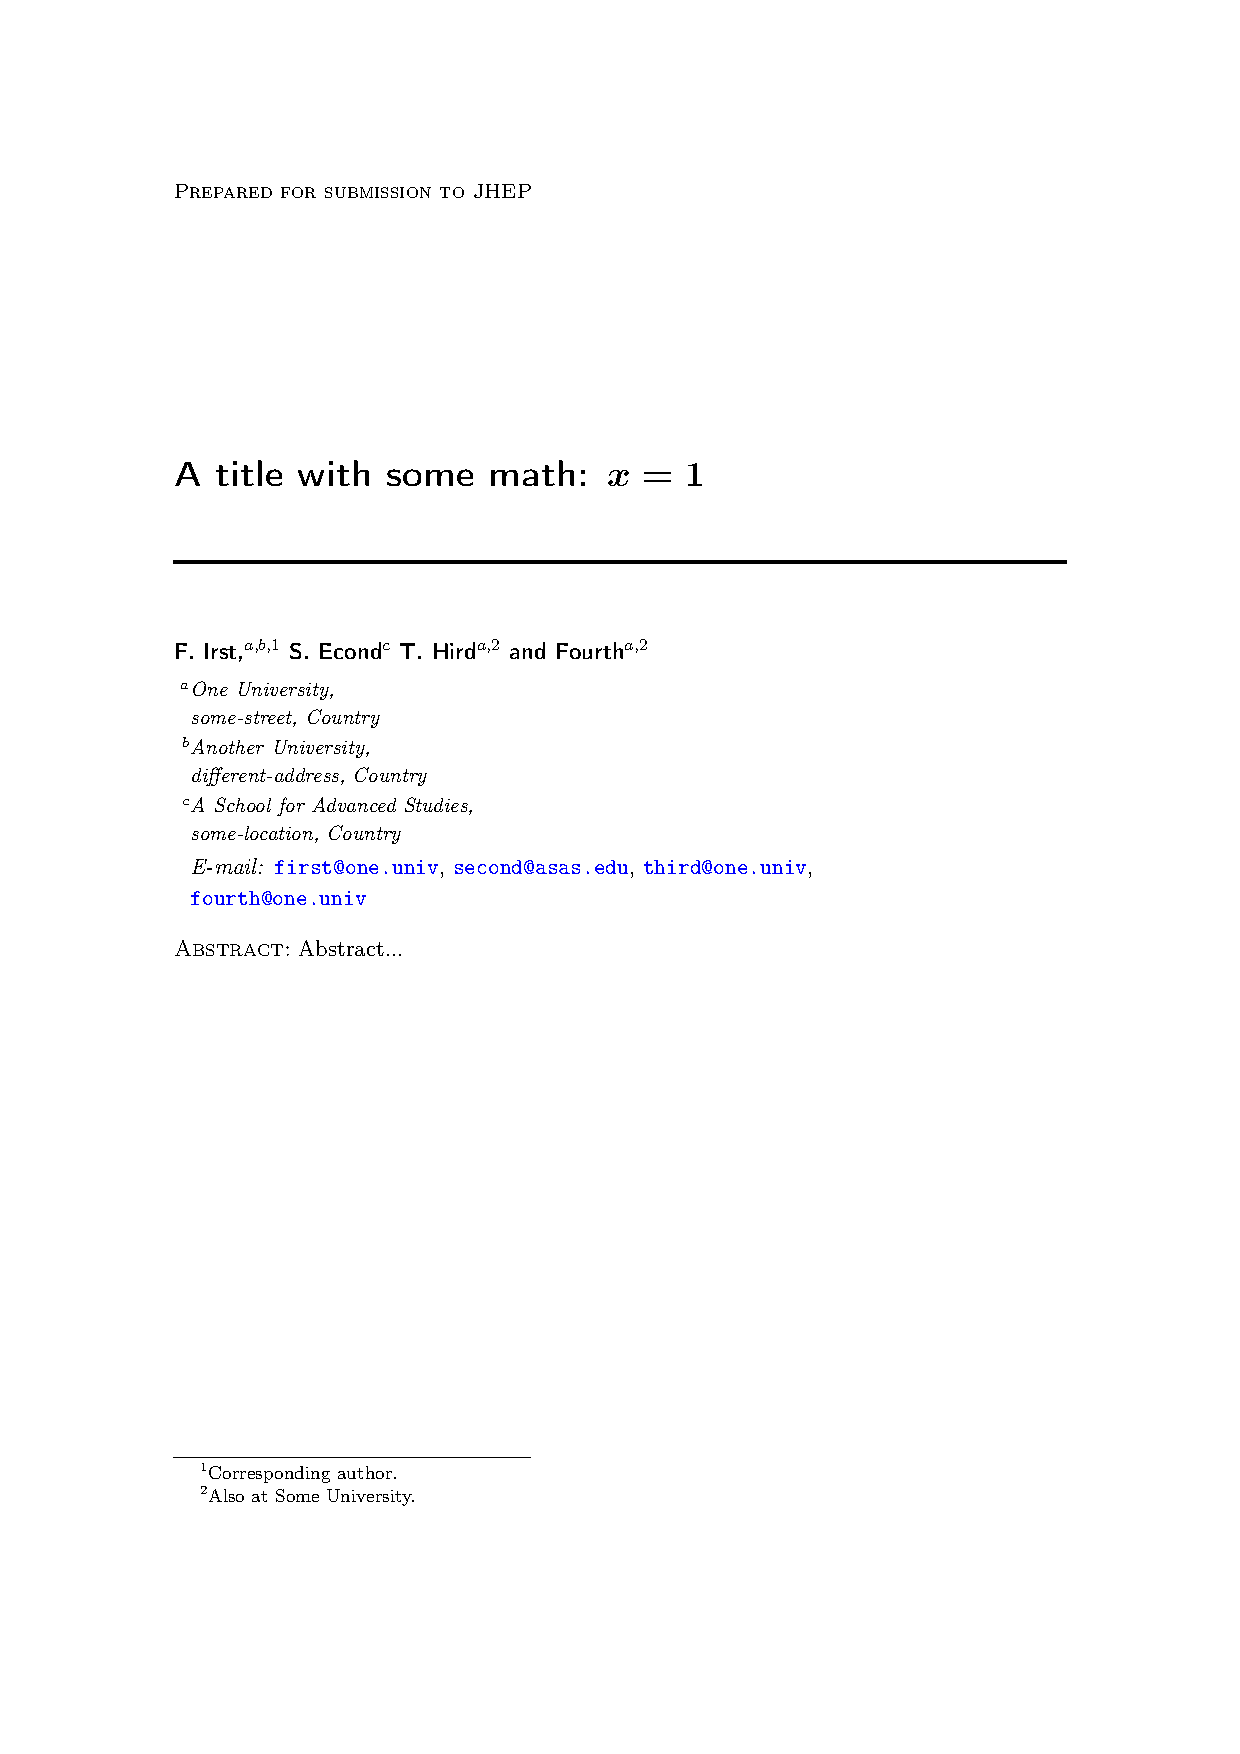
\includegraphics[width=.45\textwidth,trim=0 380 0 200,clip]{img1.pdf}
\hfill
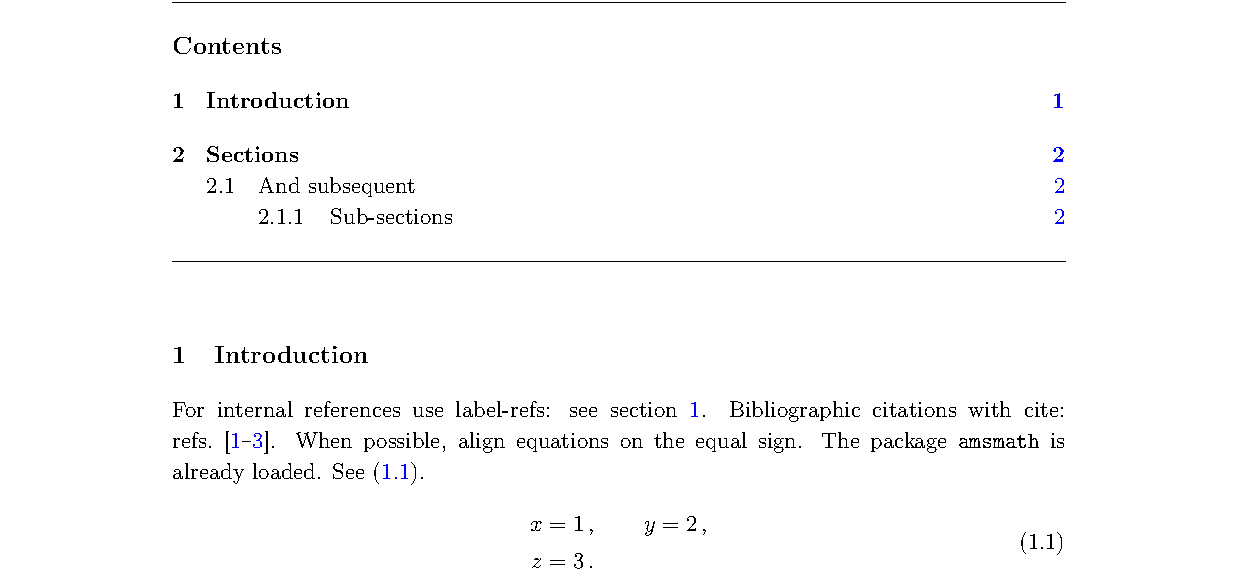
\includegraphics[width=.45\textwidth,origin=c,angle=180]{img2.pdf}
% "\includegraphics" is very powerful; the graphicx package is already loaded
\caption{\label{fig:i} Always give a caption.}
\end{figure}

\begin{table}[tbp]
\centering
\begin{tabular}{|lr|c|}
\hline
x&y&x and y\\
\hline 
a & b & a and b\\
1 & 2 & 1 and 2\\
$\alpha$ & $\beta$ & $\alpha$ and $\beta$\\
\hline
\end{tabular}
\caption{\label{tab:i} We prefer to have borders around the tables.}
\end{table}

We discourage the use of inline figures (wrapfigure), as they may be
difficult to position if the page layout changes.

We suggest not to abbreviate: ``section'', ``appendix'', ``figure''
and ``table'', but ``eq.'' and ``ref.'' are welcome. Also, please do
not use \texttt{\textbackslash emph} or \texttt{\textbackslash it} for
latin abbreviaitons: i.e., et al., e.g., vs., etc.



\section{Sections}
\subsection{And subsequent}
\subsubsection{Sub-sections}
\paragraph{Up to paragraphs.} We find that having more levels usually
reduces the clarity of the article. Also, we strongly discourage the
use of non-numbered sections (e.g.~\texttt{\textbackslash
  subsubsection*}).  Please also see the use of
``\texttt{\textbackslash texorpdfstring\{\}\{\}}'' to avoid warnings
from the hyperref package when you have math in the section titles



\appendix
\section{Some title}
Please always give a title also for appendices.





\acknowledgments

This is the most common positions for acknowledgments. A macro is
available to maintain the same layout and spelling of the heading.

\paragraph{Note added.} This is also a good position for notes added
after the paper has been written.





% The bibliography will probably be heavily edited during typesetting.
% We'll parse it and, using the arxiv number or the journal data, will
% query inspire, trying to verify the data (this will probalby spot
% eventual typos) and retrive the document DOI and eventual errata.
% We however suggest to always provide author, title and journal data:
% in short all the informations that clearly identify a document.

\begin{thebibliography}{99}

\bibitem{a}
Author, \emph{Title}, \emph{J. Abbrev.} {\bf vol} (year) pg.

\bibitem{b}
Author, \emph{Title},
arxiv:1234.5678.

\bibitem{c}
Author, \emph{Title},
Publisher (year).


% Please avoid comments such as "For a review'', "For some examples",
% "and references therein" or move them in the text. In general,
% please leave only references in the bibliography and move all
% accessory text in footnotes.

% Also, please have only one work for each \bibitem.


\end{thebibliography}
\end{document}
